% !TeX root = ../main.tex
% HLD: high level design


\chapter{概要设计}

本文需求分析章节的内容对本中文时间表达式信息抽取系统进行了详尽的需求分析,明晰了该中文时间表达式信息抽取系统需要实现的功能及其他的性能要求。
本章节将基于在第三章中分析所得的功能性需求和非功能性需求,对本中文时间表达式信息抽取系统进行概要设计,并且对该中文时间表达式信息抽取系统的整体架构以及各个模块的功能设计进行详细阐述。
通过该章节的工作内容,读者可以从总体上了解整个系统的设计思路。
本章节的工作为后续详细设计与实现做准备.

\section{系统整体架构设计}

由于笔者所在企业的开发要求, 软件系统的整体体系架构采用的是浏览器-服务器体系结构, 即B/S(Browser/Server)架构, 通过基于B/S架构的SaaS(Soft as a Service)平台向用户提供服务.
其中浏览器界面负责与客户的信息交互, 在运行时间表达式的识别和解析之前, 负责获取用户输入的语料和相关的配置等.
服务器后端开发则采用的是典型的四层架构模式, 分别为用户接口(API, Application Programming Interface)层, 外观(Facade)模式层, 服务(Service)层, 数据访问(DAO, Data Access Object)层. 详情见下图.

用户接口层是服务器端与浏览器或其他形式的数据传输方式的第一站, 用户接口层不做过于复杂的逻辑处理, 只是将系统内部提供给用户的功能暴露在外, 方便与用户交互或被开发人员调用.
在用户接口层承接网络中传入的数据, 并将其用系统内部的数据结构封装, 传递给外观模式层.

外观模式层是整个服务器后端的业务逻辑核心, 可以被认为是业务逻辑层. 外观模式获取到用户接口封装的数据结构并将其解包.
由之前的需求分析可知, 用户可能通过用户界面传入单条语句或者多条语句对中文时间表达式信息抽取系统做可行性的检验, 观察系统的输出结果,
也可能传入容量较大的文档, 或者图片以及PDF文档. 这时需要使用辅助的OCR模块对用户输入做相应的处理. 将非文字的形式转变为系统可以接受的字符串形式.
在解包用户输入以及对用户输入做预处理后, 这些数据将被中文时间表达式识别模块接收.
中文时间表达式模块会根据底层的基本元素组合出规则, 通过规则匹配的形式将中文时间表达式这一类实体从起来源的语料中提取出来, 然后将其抽象化为特殊的元素形式, 最后将这些元素提交给中文时间表达式解析模块.
中文时间表达式解析模块将识别模块识别出的元素作为叶结点, 自下而上的构建出一棵或多棵语法树, 当出现多棵语法树时, 将通过朴素贝叶斯选择器模块进行辅助, 判断决策采用哪一棵树作为最终生成的结果树.
结果树在解析的过程中会被自然的携带结构化的时间信息, 最终在根结点可以直接格式化为UTC形式的时间.

服务层主要负责和数据库交互的服务逻辑, 负责将外观模式层的处理结果最终保存到数据库中进行持久化.
如果没有服务层作为数据库与业务逻辑之间的桥梁, 那大量有价值的原始语料或解析结果将不复存在.
服务层会对数据库中的操作进行简单的聚合, 完成较为复杂的数据存取操作.

数据访问层是对数据库表中行记录的具现化, 是对象关系映射模型(ORM, Object Relation Mapping)的具体实现, 数据访问层详细的表示了数据库中存储的行记录中各个字段或属性的名称以及类型.
为服务层针对数据库表的操作提供了一定的便捷性.

此外, 为了方便用户进行批处理, 即传入大量的文档或图片. 本中文时间表达式信息抽取系统采用分布式的方法来优化批处理任务.
系统内部一共部署了六台逻辑服务器, 其中三台运行中文时间表达式信息抽取系统, 用作任务服务器, 一台服务器专做数据库服务器, 以存储中间数据, 一台服务器作为静态资源服务器, 一台服务器作为反向代理服务器.
三台任务服务器都使用多线程的方式运行中文时间表达式信息抽取系统, 而代理服务器采用复杂均衡的方式将用户请求产生的负载较为均匀的分配在三台任务服务器上. 复杂均衡的分布式运算使得批处理的时间大大剪短.
中文时间表达式信息抽取系统的网络拓扑图如下图所示.


\section{系统功能模块设计}

在制作中文时间表达式信息抽取系统的功能结构善主要参照的原则是:
在模块的内部高度集聚,每个模块之间的连接性不高的原则,和固有的制作软件的要求一样,将相互管理
的模块进行合并,然后对相互的数据进行转换.
在系统内部,并未划分一个独立的方面来进行数据的交流转换,在这样的区别之后,能够更加方便的完成吸引的功能,按照每个方面彼此之间的关联,可以使各个子系统分层次的进行制作和开发,使用调用的形式来完成每个模块的要求。
利用系统整体架构设计中提到的用户接口层、外观模式层、服务层, 数据访问层四者者之间的联系来对子系统进行划分。
在单独制作模块的过程中,使用单独的制作来完成功能,确保每个用户功能的单独性,不会因为极小的变动就会影响全局,使系统的更新和改善互相独立,使系统更加的安全。
使用模块的划分来展示系统的作用来进行相应的开发。


\subsection{中文时间表达式识别模块}

当用户进入浏览器中, 系统用户界面会默认给用户提供输入为普通文本的选项. 如果用户需要修改自己的输入为PDF文档或者图片时, 可以显示的将输入修改为PDF文档或图片.
中文时间表达式识别模块在接收到上层用户接口传入的封装数据后, 将会根据文件本身的格式和用户选择的输入配置决定对文件的解析方式. 如果解析成功则顺利进入下一步识别的流程.
否则将会单独标识文件处理错误, 并向用户告知这一文件解析方式存在问题, 提醒用户更改输入配置.
如果文本类型为JSON, CSV或TXT格式, 那么将会直接进入后续的文本预处理流程.
在根据文件格式和用户输入配置得知文件类型为PDF文档或图片格式时, 中文时间表达式识别模块将该文件委托给OCR识别模块进行识别. 识别的结果将会返回后续的文本预处理流程.
在初步得到文本文件后, 需要使用与文本预处理模块对文本中含有的表情, 全半角符号或者转义符号做一定的处理, 防止后续的识别过程识别到错误的实体.
当文本文件经过预处理后, 将会同时被数字类型识别模块和时间单元识别模块同时处理.
数字类型识别模块将通过正则匹配的形式匹配到文本中所有的中文或英文数字, 并将其封装成数字类型基本元素对象.
而时间识别单元也是通过正则匹配的形式匹配到文本中所有的中文形式的时间单元, 并将其封装为时间类型基本元素对象.
这些识别到的对象会根据在文本中出现的顺序进行排序, 并交付给中文时间表达式解析模块进行解析.

\subsection{中文时间表达式解析模块}

如果系统内部还没有朴素贝叶斯选择器的模型参数, 将会首先读取语料库中的所有语料, 根据事先已经标注好的训练集做简单的预料训练.
中文时间表达式解析模块首先将系统内部定义好所有基本元素对象按照事先已经定义好的规则进行组合, 然后调用上文中所述的中文时间表达式识别模块进行识别.
规则识别模块将识别出的基本元素需要按照上下文无关语法的产生式进行反向推到, 用以得到所有的推导规则.
统计每一个推导规则在整个语料中识别出的所有规则的概率值, 以此值作为似然记录下来. 待到所有的推导规则似然值的统计完毕, 即可组建似然函数.
此后解析树构建模块按照概率无关上下文语法将, 通过中文时间表达式识别模块的得到的用户输入产生的基本元素, 通过规则组合模块处理得到的一系列规则,
按照每个规则的似然值, 自下而上的构建出一棵或多棵语法树.
如果在构建树的过程中出现了冲突, 那么冲突消解模块会根据似然函数进行冲突消解.

\subsection{信息抽取系统分析结果与语料存取模块}

信息抽取系统分析结果与语料存取模块主要负责中文时间表达式信息抽取系统中将分析结果和语料存入到数据库中.
用户传入的语料首先会生成对应的序列号, 进行唯一标识, 然后存入数据库中.
如果用户传入的类型为PDF文档类型或图片类型, 则为文件资源生成唯一标识码, 并将该文件类型重命名为唯一标识码, 存放到系统指定位置.
随后语料会经过识别和解析两个模块, 生成最终的结果.
信息抽取系统分析结果与语料存储模块将该结果按照序列号存入对应的行记录中, 此时需要按照开发人员提前配置好的文件, 决定最终录入数据库中数据的大小.
最终结果需要包含识别到的实体, 实体边界还有相应的语法分析树.
当开发人员需要读取语料或者用户需要分析结果, 此时信息抽取系统分析结果与语料存取模块需要读取用户传入或开发人员定义好的配置, 从数据库中取出相应的数据,
交付给信息抽取系统分析与展示模块进行展示.

\subsection{信息抽取系统分析与展示模块}

信息抽取系统分析与展示模块通过Metis面板读当前数据分析需求向后台的MongoDB数据库进行SQL语句查询请求, 并且将查询结果以可视化的方式显示到Metis面板智商.
图4.3是信息抽取系统分析与展示模块的活动图, 该图描述了信息抽取系统分析与展示模块的各项功能, 当前改模块一共进行10个查询需求, 下面对每一项功能进行详细的说明.

\begin{enumerate}
  \item[(1)] 每日表达式识别失败数量

    每日表达式识别失败数量查询需求可以通过在数据库表的时间戳字段上建立索引, 并且通过查询数据库表上每个行记录识别失败总量之和, 即可得出每日表达式识别失败总量.

  \item[(2)] 每日表达式解析失败数量

    每日表达式解析失败数量查询需求可以通过在数据库表的时间戳字段上建立索引, 并且通过查询数据库表上每个行记录解析失败总量之和, 即可得出每日表达式解析失败总量.

  \item[(3)] 每日表达式识别与解析用户调用数量

    每日表达式识别与解析用户调用数量查询需求可以通过在数据库表的时间戳字段和用户唯一标识字段建立索引, 并且通过查询数据库表上当天每用户查询总量, 即可得出每日表达式识别与解析用户调用数量.

  \item[(4)] 每日OCR模块调用总量

    每日OCR模块调用总量可以通过在数据库表的时间戳字段上建立索引, 并且根据行记录的文件类型是否为PDF文档或图片类型进行计算, 即可得出每日表达式识别与解析用户调用数量.

  \item[(5)] 每日表达式识别失败分析

    每日表达式识别失败分析可以通过在数据库表的时间戳字段上建立索引, 并且根据行记录中的失败记录和中文时间表达式解析树进行分析, 即可得到每日表达式识别失败分析.

  \item[(6)] 每日表达式解析失败分析

    每日表达式识别失败分析可以通过在数据库表的时间戳字段上建立索引, 并且根据行记录中的失败记录和中文时间表达式解析树进行分析, 即可得到每日表达式识别失败分析.

  \item[(7)] 单语句可视化分析

    单语句可视化分析可以通过在数据库表的时间戳字段上建立索引, 并且根据行记录中的中文时间表达式解析树进行分析, 即可得到单语句可视化分析.
\end{enumerate}

\begin{figure}[h]
  \centering
  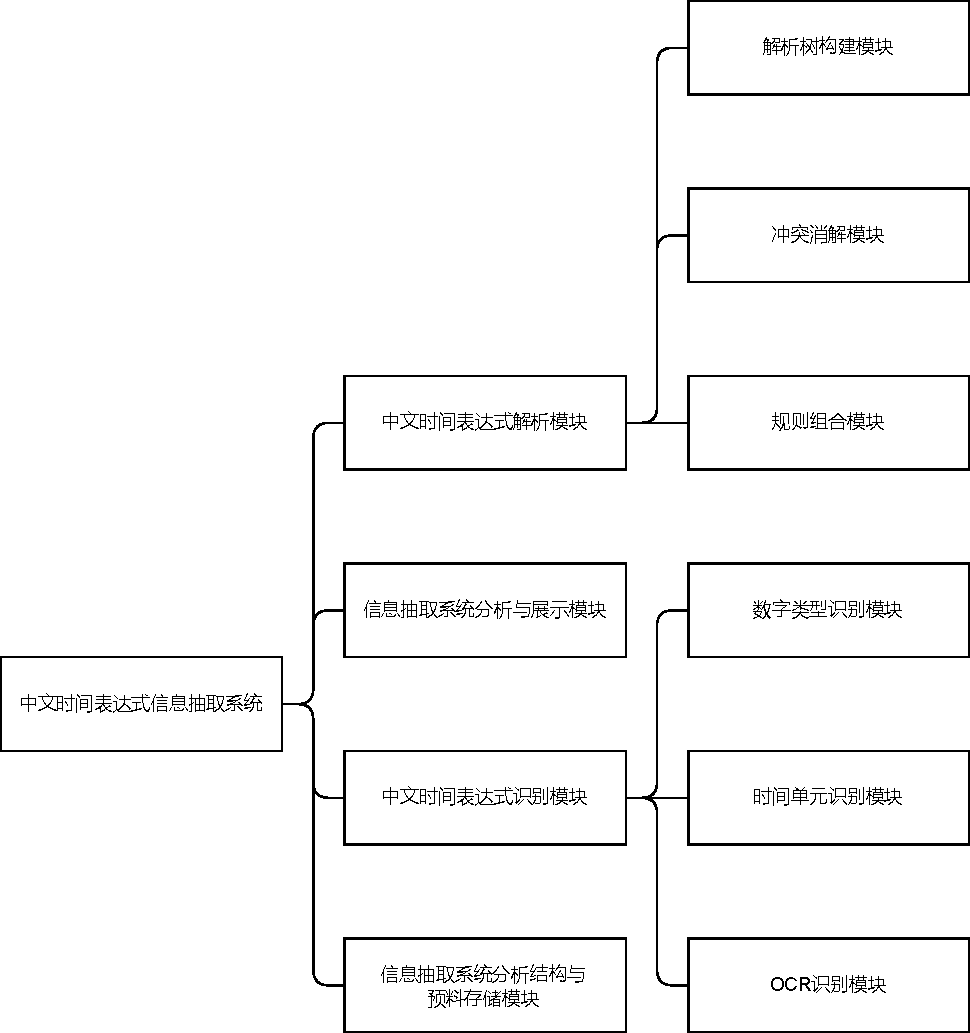
\includegraphics[width=1\textwidth]{系统功能模块.pdf}
  \caption{系统功能模块图}
  \label{fig:badge}
\end{figure}

\section{数据库设计}

数据库是本系统的重要组成部分, 主要负责中文时间表达式信息抽取系统中导出数据的持久化存储方面的工作.
数据库及相关数据表的设计也是软件开发工程里设计流程中非常关键的步骤之一, 因为数据库的设计关系到上层查询接口的易用性, 查询效率以及数据的完整性和一致性, 是保障数据存储效率和数据完整安全的重要环节.
因为中文时间表达式信息抽取系统大量的使用文本类型数据, 数据的JSON化程度较高. 在当前众多的开源数据库中, 非关系型数据库(NoSQL, Not-only SQL)是比较适合存储这类大文本类型的数据的.
其中MongoDB又是特意为文本存储设计的键-值对数据库, 是一款拥有高兴能的数据库管理系统, 因此本中文时间表达式抽取系统底层采用MongoDB进行数据持久层的开发.

\begin{table}[h]
  \centering
  \caption{数据库表结构设计}
  \begin{tabular}{|*{7}{c|}}
    \hline
    序号 & 字段名          & 字段说明                 & 类型    & \makecell*[c]{是否                                              \\为空} & 说明                  & 默认值        \\
    \hline
    1    & uid             & 用户号                   & String  & 否                 & \makecell*[c]{PK(uid, sid,                 \\doc\_id)} & “0”           \\
    \hline
    2    & sid             & 流水号                   & String  & 否                 & \makecell*[c]{PK(uid, sid,                 \\doc\_id)} & “0”           \\
    \hline
    3    & create\_date    & 创建时间戳               & Date    & 否                 & null                       & CURRENT\_DATE \\
    \hline
    4    & doc             & \makecell*[c]{用户                                                                                   \\导入语料} & String  & 否       & null                  & “0”           \\
    \hline
    5    & doc\_id         & 文档号                   & String  & 否                 & \makecell*[c]{PK(uid, sid,                 \\doc\_id)} & “0”           \\
    \hline
    6    & doc\_num        & 文档序号                 & Integer & 否                 & null                       & "0"           \\
    \hline
    7    & result          & 解析结果                 & String  & 否                 & null                       & “0"           \\
    \hline
    8    & real\_num       & \makecell*[c]{应该识别                                                                               \\及解析个数} & Integer & 否 & null & 0 \\
    \hline
    9    & resolution\_num & \makecell*[c]{实际正确                                                                               \\解析个数} & Integer & 否 & null & 0 \\
    \hline
    10   & reconition\_num & \makecell*[c]{实际正确                                                                               \\识别个数} & Integer & 否 & null  & 0 \\
    \hline
    11   & label           & \makecell*[c]{识别及解析                                                                             \\标定结果} & String & 否 & null & “0” \\
    \hline
  \end{tabular}
\end{table}

\section{本章小节}

本章节主要从中文时间表达式信息抽取系统的整体设计入手, 详细介绍了本信息抽取系统的整体架构.
信息抽取系统主要分为四个模块: 信息抽取系统分析结果与预料存储模块, 中文时间表达式识别模块, 中文时间表达式解析模块以及信息抽取系统分析与展示模块, 并分别对上述模块的功能尽心了阐明, 设计并展示了各个子模块的活动图.
其中中文时间表达式识别和解析模块内部又存在多个相辅相成, 互相作用的子模块. 本章内容详细介绍了本信息抽取系统的整体设计以及功能模块设计.
最后, 本系统还使用了数据库存储系统用以存取解析结果, 对解析结果的数据结构及其春初进行了设计. 本章的概要设计工作为本中文时间表达式信息抽取系统的详细设计与实现提供了方向.

